\part{Results}
\chapter{Results}
\section{Imaging live cells}
For the study described in \textbf{Paper I} we used cells of two species of cyanobacteria as a sample: Cyanobium gracile and Synechococcus elongatus. Cyanobacteria are photosynthetic bacteria that can be found in almost any habitat on earth, ranging from hot volcanic areas to cold polar ice caps, and play an important role in the global carbon and nitrogen cycle. In a 25 day cycle an algal bloom of 1000 $km^2$ can sequester around 22,000 tonnes of atmospheric carbon into organic carbon before an infection by cyanophages caused the bloom to collapse.
 
Cyanobium gracile cells were selected for their small size and their robustness with respect to the injection procedure. Solitary C. gracile and S. elongatus cells have an oval-to-cylindrical shape, and vary in size between 0.25-0.4 $\mu$m in diameter and 0.4-4.0 $\mu$m in length \cite{Komarek1999}. Cells divide symmetrically by binary fission. The two daughter cells separate from each other after reaching the size and shape of the mother cell \cite{Bazire1988}. We used non-synchronised cell cultures undergoing active growth which provided cells in various stages of their cell cycle. 

The experiments described in \textbf{Paper I} were carried out at the atomic, molecular, and optical science (AMO) endstation at LCLS \cite{Bostedt2013}, at 512 eV (2.40 nm) and 1100 eV (1.13 nm) photon energy.  Figure \ref{fig:ExperimentalSetup} shows the arrangement of the experiment. The length of the photon bunch was about 70 fs. Far-field diffraction patterns were recorded on a pair of pnCCD detectors \cite{Struder2010} in the CFEL-ASG Multi Purpose (CAMP) instrument \cite{Struder2010}. The detectors were place at 741 mm downstream from the interaction region of the beam and the sample. The detector read out rate matched the 120 Hz repetition rate of the LCLS. 

We collected diffraction patterns of C. gracile cells for an hour at a hit ratio of 43\%. Over 7,500 clear hits were selected for further analysis, using the Cheetah software package \cite{Barty2014}. The linear sampling ratio of the particle was around 20-fold, which allowed direct phase recovery from the measured intensity patterns. Phase retrieval was not a trivial problem because strong hits saturated the detectors at low diffraction angles. As a compromise, we manually selected medium-strong hits, which contained either no, or only few saturated pixels, while still providing scattered signal to reasonably high resolution. Missing mode analysis revealed no unconstrained modes for all reconstructed cells presented in \textbf{Paper I}. 

Phases were retrieved using the Hawk software package \cite{Maia2010}. For each pattern 400 reconstructions were made, each starting from different random initial phases. These reconstructions consisted of 5000 iterations with the RAAR algorithm \cite{Luke2005}, using a Shrinkwrap algorithm \cite{} for support determination, and concluded with 100 iterations by the ER algorithm \cite{Fienup1978, Fienup1982}. The initial and final support size was selected manually. No additional constraints were used since we anticipated the effects of absorption in the thick cells to give effects similar to a phase object. 

Figure \ref{fig:Reconstructions} shows the reconstructed exit wave-fronts (images) for six live C. gracile cells together with the corresponding diffraction patterns, and a synthetic Nomarski image. The reconstructions represent 2D projections of the electron density of the cells. The images show the expected morphologies of cells during division \cite{Komarek1999,Bazire1988}. The resolution of each  reconstruction is indicated by the size of the round white dot. Features smaller than the dot need to be interpreted with care.

Resolution for the reconstructions was estimated from the PRTF (See Figure \ref{fig:ExperimentalSetup}), using the 1/e cut-off. Before calculating a PRTF and averaging the images we removed outliers among the reconstructions by applying a threshold to the Fourier error. Clustering validates the results from using a threshold on the Fourier-Error and the real-space error(Figures 7 a-j). On average the main cluster contained about 370 out of 400 reconstructions (93\%), except for one case where only 96 reconstructions formed the biggest cluster (Figure 7j). This made us believe that the average image of the main cluster is the true reconstruction minimum. Th failed reconstructions did not find the true minimum.
The scatter plots of Figure 7 a-j show that the real-space error is more reliable than the Fourier-error for identifying failed reconstructions.

Detector saturation limited the achievable resolution.  In fact, the reconstructions shown in Figure \ref{fig:ExperimentalSetup} come from exposures that did not saturate the detectors. A number of much stronger exposures were also recorded, and in some of these exposures the diffraction signal extended to nanometer resolution. Figure \ref{fig:StrongHit} shows one such pattern for a live S. elongatus cell at 1,100 eV photon energy, 70 fs pulse length, about $10^11$ photons $\mu m^{-2}$ on the sample. Two pnCCD detector pairs were used to record this pattern. The configuration of the central back detector in Figure  is identical to the detector used in Figure \ref{fig:ExperimentalSetup}. The front detector is the same type as the back detector but is placed at 220 mm from the interaction region. In this strong hit, a large part of the back detector was saturated, preventing reliable phasing. The signal however extended beyond 4 nm resolution on the front detectors (at sigma 3.7), which is the size of a small protein molecule. More than 58 million scattered photons were recorded on the back detectors, and 1.3 million on the front detectors. The size of the cell was derived from the autocorrelation. Figure 4c shows that in a log/log representation the drop-off of the signal is linear with spatial frequency in the range covered by our measurements, and the exponent of the signal decay is $-3.31\pm0.01$, matching simulations \cite{Huang2009}.



\section{Classification}

Given the high data rates of XFELs it is impossible for humans to go through all data frames individually, and assistance of computers is needed.
RedFlamingo is a software framework designed to rapidly assess individual diffraction patterns by reducing their complexity to a small set of interpretable numbers. The power of RedFlamingo lies in its modularity: users have the option to select a combination of algorithms they want to use for data evaluation, and can port their own algorithms. This is important, as each sample and experiment will come with its own set of demands on data analysis. For example the number of scattered photons vary considerably from sample to sample. This will affect the way diffraction patterns can be evaluated. Furthermore, the detector type often changes from experimental station to experimental station, and each experiment has its own specific artefacts due to the experimental condition at the time of operation. Within this variation it is very important to be able to know whether or not you are imaging the particle of interest, at what rate, and if it is intact. For deeper data analysis one often needs to limit the amount of heterogeneity within the data to an even larger extend. This makes is very difficult to design algorithms that are useful for every data set. RedFlamingo will make it possible to combine algorithms from different experiments, each often designed to tackle a specific problem. 

RedFlamingo has been tested on several datasets. This chapter shows four cases that illustrate different demands on the data analysis. In the first example, RedFlamingo is used for pattern classification. The main discriminatory features were size, particle elongation, and number of particles in the beam. The second example shows that RedFlamingo can be used to size particles within a wide range of sizes and shapes. The third example shows diffraction patterns from single particles can be separated from diffraction patterns originating from multiple particles located at a distance from each other. The final example shows how the shape of elongated particles can be determined more carefully. 

\subsection{Pattern Classification of heterogeneous RDV data set}
Rice Dwarf Virus (RDV) is the causal agent of rice dwarf disease. It can result in severe crop losses in rice and other gramineae plants in East Asian countries due to stunted growth and chlorotic specks. The structure of RDV has previously been solved to 3.5 $A$ resolution by X-ray crystallography \cite{Nakagawa2003} (PDB 1UF2). RDV is approximately 72 nm in diameter across the 5-fold axis.

Most diffraction patterns in this data set are not affected by detector saturation, which makes it possible to estimate the size of the icosahedral-shaped particle by determining the location of the first minima (see chapter 7).
RDV was classified on the size and shape of the central speckle, and the size and shape of the central term in the autocorrelation. If the central speckle and the central term of the autocorrelation are circular to slightly elongated the particle was classified as a single particle.  
The patterns that are showing interference signal, origination for multiple particles are also grouped together.

\begin{figure}[h]
\centering
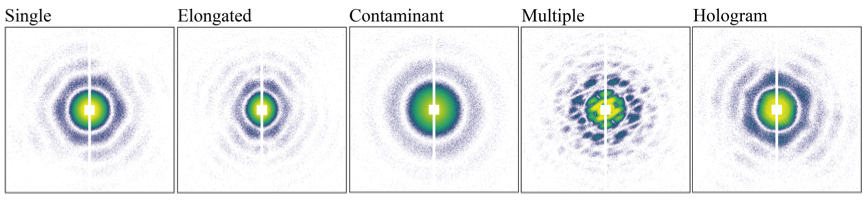
\includegraphics[width=100mm]{Chapter_09_Results_RDV_classes.png}
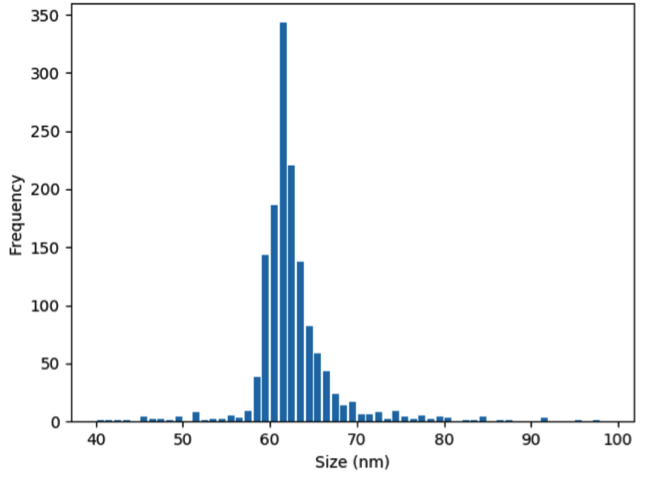
\includegraphics[width=100mm]{Chapter_09_Results_RDV_size_distribution.png}\label{fig:Classes}
\caption{Classification of particles. Top: one example pattern from each class is shown. The gap between the two detector halves and the beam stop is masked out. Bottom: the size distribution of the 3608 diffraction patterns classified as single hits shows a peak at 63 nm.}
\end{figure}

The diffraction patterns that have a round central speckle show features commonly associated with icosahedral particles. Surprisingly, the mean size of these particles is smaller then the expected size of the RDV particles. It has been observed more often that the size estimation of particles is consistently 10 \% - 15\% smaller than their size measured by other measures. This could have to with uncertainties in the actual wavelength or detector distance, or possibly by another cause. 


\subsection{Pattern Selection based on edges}
The second example deals with the selection of diffraction patterns based on the presence of sharp edges. The sample that was used is the 331-kbp chlorovirus Paramecium bursaria chlorella virus 1 (PBCV-1). PBCV-1 is the type member of the genus Chlorovirus (family Phycodnaviridae) that infects certain chlorella-like green algae from freshwater sources \ref{Nagakawa, VanEtten2012}. It is a quasi-icosahedral particle with a diameter of 190 nm across the 5-fold axis  One of the PBCV-1 vertices has a 56 nm long spike structure; 34 nm protrudes from the surface of the virus.

In the experiment PBCV particles were injected into the XFEL focus using a GDVN. This resulted in a wide size distribution, of which elongation assessment showed that most particles are very round. Using the streak finding algorithm described in Chapter 8, we could fine patterns that show clear streaks (See figure \ref{fig:PatternSelection}


\subsection{Multiple Located At a Distance}

In the experiment such as described by Paper XX, Xenon droplets of approximately 70 nm in diameter are injected together with the biological sample, but using a different injection procedure. If a drop and particle are imaged simultaneously (or any combination, such as drop-drop or particle-particle), a diffraction pattern similar to Figure \ref{fig:multiplefinding} will be measured. To sort out the patterns with and without interference structure, the algorithm described in Chapter 8 can be used. Table \ref{tab:multiple_find} shows the results of the classification method, for samples of varying between 70 and 1000 nm in size. The diffraction patterns of the smallest sample (70 nm) came from a different experiment in which the sample was not co-injected with Xenon droplets. Therefore the fraction of normal vs. multiple patterns is much lower. Also the xenon injection sample 2 is less successful than that of sample 1 and sample 3-4.

\begin{figure}[h]
\centering
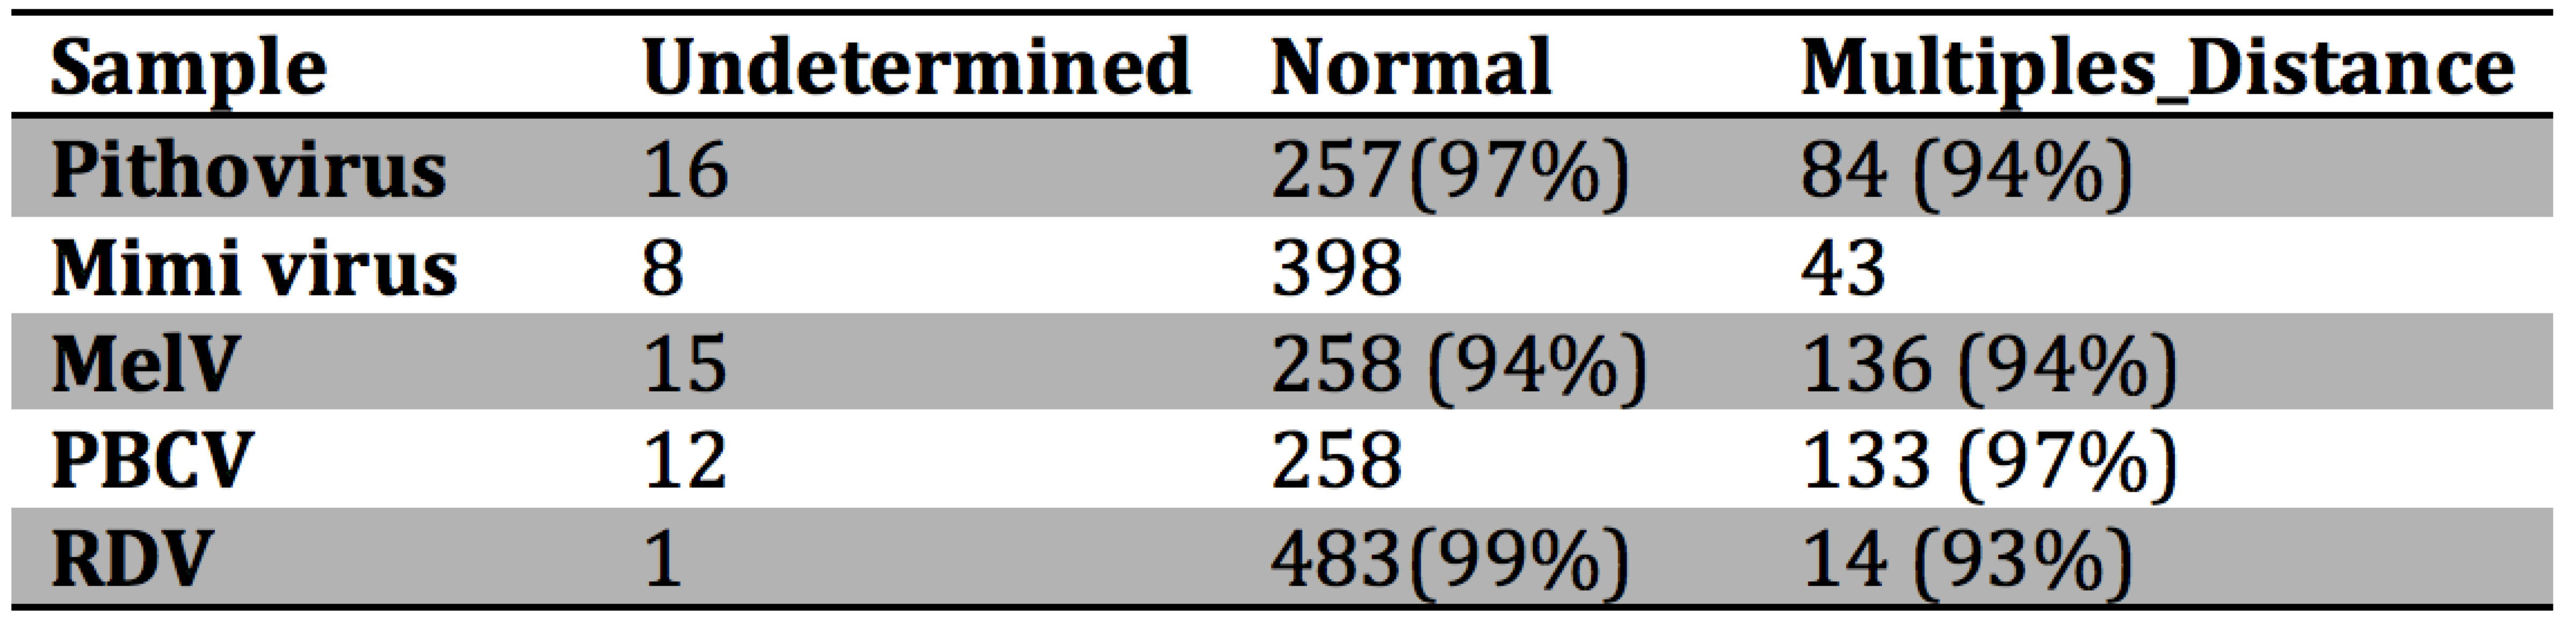
\includegraphics[width=100mm]{Chapter_09_Results_successrate.png}
\label{fig:Classes}
\caption{Determination of multiple particles in the focus. Diffraction patterns from five different samples ranging from > 1000 nm to 70 nm in size were classified as coming from multiple particles at the same time. There are three classes: MultipleDistance, Normal, and Undetermined. Patterns with strong saturation are put in the latter class, because the autocorrelation sometimes shown strong artefacts because of it. }

\end{figure}

\section{Software}

